\chap{Conclusion}

\section{Summary}

\section{Recommendations to future work}

\subsection{Dataset about single locality}
This thesis allows to have a general overview and predictions of values about the aquaculture business in Norway. 

But it would be much more useful, in particular for people into the aquaculture business, to use this system to have an overview and predictions of data provided by a single locality of aquaculture.\\
In this case the system could be used from the owner of the locality to analyze historic values and use the prediction system to have a forecast about some particular parameters.

\subsection{Visualization of the data}

\subsection{Test prediction system with a bigger dataset}

\section{Prediction system as a service}
This system has been developed with the idea that it could become a "Service system", that is basically a configuration of technology and organizational networks designed to deliver services that satisfy the needs or wants of customers.
Since the prediction system implemented during this work is almost 100\% reusable, it could be used from people for prediction about any kind of data. 

Basically the idea is to create a web application that allows to let you upload your own dataset, choose your own preferences and prediction settings, and then the system will calculate and display prediction of the current values in the future together with the MAPE (Mean Average Percentage Error) to have an idea bout how accurate are the.\\


\begin{figure}[H]
	\centering
        \makebox[\textwidth][c]{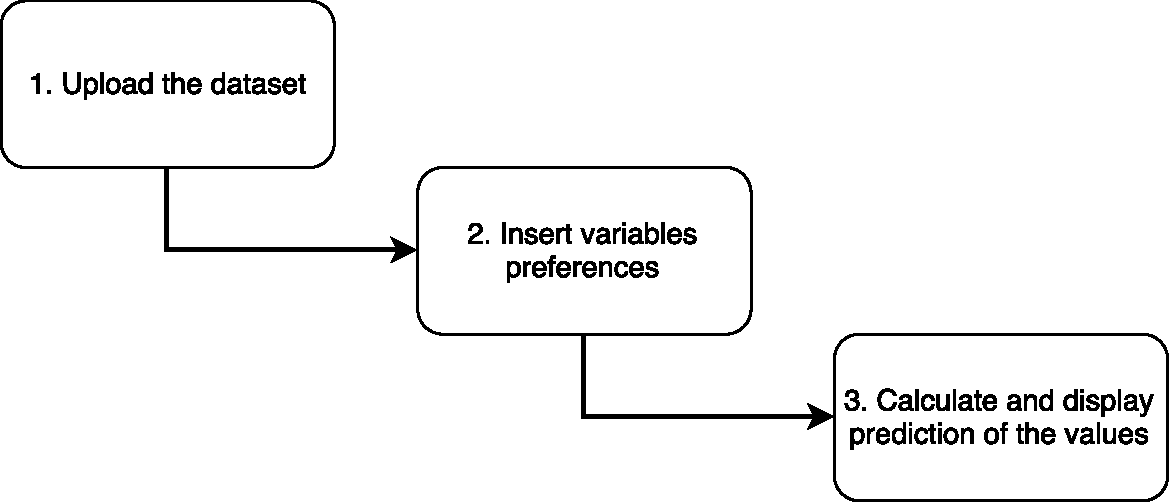
\includegraphics[width=1\textwidth]{Files/ServiceSystem.pdf}}
    \caption{Idea of the Servie System for predictions.}
\end{figure}






